\documentclass[conference]{IEEEtran}
% *** GRAPHICS RELATED PACKAGES ***
%
\ifCLASSINFOpdf
  \usepackage[pdftex]{graphicx}
  % declare the path(s) where your graphic files are
  % \graphicspath{{../pdf/}{../jpeg/}}
  % and their extensions so you won't have to specify these with
  % every instance of \includegraphics
  \DeclareGraphicsExtensions{.pdf,.jpeg,.png}
\else
  % or other class option (dvipsone, dvipdf, if not using dvips). graphicx
  % will default to the driver specified in the system graphics.cfg if no
  % driver is specified.
  \usepackage[dvips]{graphicx}
  % declare the path(s) where your graphic files are
  % \graphicspath{{../eps/}}
  % and their extensions so you won't have to specify these with
  % every instance of \includegraphics
  % \DeclareGraphicsExtensions{.eps}
\fi

\usepackage{pgf}
%\usepackage{tikz}
%\usetikzlibrary{arrows,automata}

\definecolor{darkgreen}{rgb}{0,0.7,0}

\newif\ifdraft
\drafttrue
%\draftfalse
\ifdraft
 \newcommand{\katznote}[1]{ {\textcolor{blue} { ***Dan:   #1 }}}
 \newcommand{\ketanote}[1]{{\textcolor{orange}  { ***Ketan:   #1 }}}
 \newcommand{\kriedernote}[1]{ {\textcolor{darkgreen}  { ***Scott:   #1 }}}
 \newcommand{\note}[1]{ {\textcolor{red}    {\bf #1 }}}
\else
 \newcommand{\katznote}[1]{}
 \newcommand{\kriedernote}[1]{}
 \newcommand{\note}[1]{}
\fi
% correct bad hyphenation here
%\hyphenation{op-tical net-works semi-conduc-tor}

\hyphenation{Queuing}

\begin{document}
%
% can use linebreaks \\ within to get better formatting as desired
\title{Accelerating Scientific Workflow Applications with GPUs}

%\author{\IEEEauthorblockN{Auth1\IEEEauthorrefmark{1},
%Auth2\IEEEauthorrefmark{1}\IEEEauthorrefmark{1}, 
%Auth3\IEEEauthorrefmark{1},
%\IEEEauthorblockA{\IEEEauthorrefmark{1}Argonne National Laboratory}
%}}

\author{Dustin Shahidehpour\IEEEauthorrefmark{1},
Scott J. Krieder\IEEEauthorrefmark{1},
Jeffrey Johnson\IEEEauthorrefmark{1}\\
Benjamin Grimmer\IEEEauthorrefmark{1},
Justin M. Wozniak\IEEEauthorrefmark{2},
Michael Wilde\IEEEauthorrefmark{2}\IEEEauthorrefmark{3},
Ioan Raicu\IEEEauthorrefmark{1}\IEEEauthorrefmark{2}\\
\IEEEauthorblockA{
\IEEEauthorrefmark{1}Department of Computer Science, Illinois Institute of Technology}
\IEEEauthorrefmark{2}MCS Division, Argonne National Laboratory\\
\IEEEauthorrefmark{3}Computation Institute, University of Chicago
}


\maketitle


\begin{abstract}
This work analyzes the performance increases gained from enabling Swift applications to utilize the GPU through the GeMTC Framework. By identifying computationally intensive portions of Swift applications, we can easily turn these code blocks into GeMTC microkernels. Users can then call these microkernels throughout the lifetime of their Swift application. The GeMTC API handles task overlap and data movement, providing transparent GPU acceleration for the user. This work highlights preliminary performance results from the scientific application MDProxy. This application determines the energy of particles in a modeled universe as they move around in space.
\end{abstract}

% no keywords
\begin{IEEEkeywords}
Many-Task Computing, Swift, GPGPU, CUDA
\end{IEEEkeywords}

\IEEEpeerreviewmaketitle

\section{Background Information}
GeMTC (GPU enabled Many-Task Computing) \cite{kriederSC12}, is a CUDA-based framework which provides efficient support for Many-Task Computing \cite{raicu2008toward} workloads on accelerators. \cite{kriederGCASR12} The GeMTC framework has been integrated into Swift/T \cite{wozniak13swift}, a parallel programming framework from Argonne National Laboratory and the University of Chicago, providing GPU functionality for the Swift language. \cite{zhao2007swift}

A microkernel is a traditional CUDA kernel that is modified to run in the GeMTC framework. A CUDA kernel is a user-defined function that runs on a NVIDIA GPU.

\section{MDProxy Architecture}
In Figure \ref{fig:md_proxy_arch} the call stack architecture is shown for MDProxy through Swift and GeMTC. The user writes a Swift script that will build an array of potential particles and calls GeMTC MDProxy with this array as a parameter. Each call to MDProxy creates it's own universe of particles and ships the universe to the GPU. Finally the MDProxy application consists of three functions 1) initialize the universe, 2) run the computation, and 3) update the result.

\begin{figure}[h]
\centering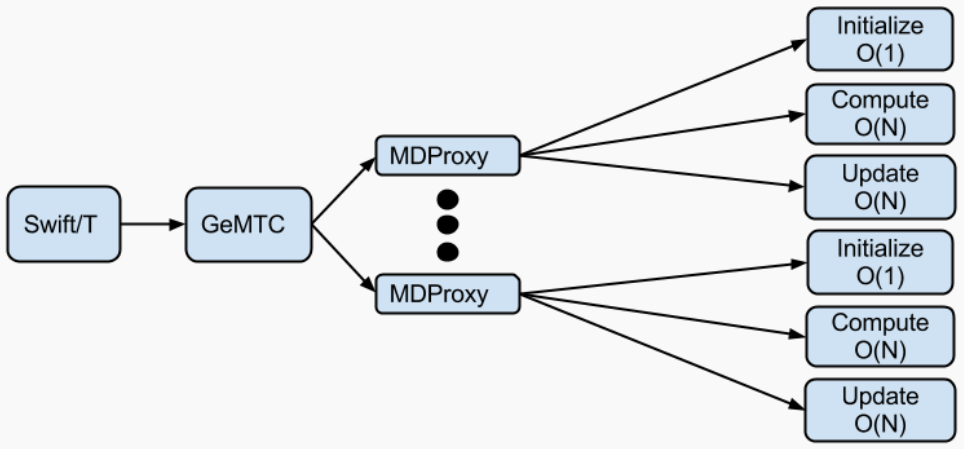
\includegraphics[width=8cm]{imgs/md_proxy_arch.png}
\caption{Call stack architecture for the MDProxy implementation.}
\label{fig:md_proxy_arch}
\end{figure}


\section{Testing Environment}
In this work we conduct our evaluation on a GTX 670 GPU with 7 Streaming Multiprocessors (SMXs). In addition this GPU contains 84 Warps(utilized as workers), 1344 CUDA Cores, and 2GB of DDR5 RAM. CPU results are tested on a 6 core 3Ghz AMD CPU.

\section{MDProxy Evaluation}

In Figure \ref{fig:cpu_gpu} the GeMTC MDProxy micro-kernel is evaluated with 2,688 particles and scaled up to 900 steps of computation from within the application. In addition, a comparison is drawn against a threaded CPU implementation of MDProxy with the GPU version showing a 10x speedup. Finally, Figure \ref{fig:tasks_per_sec} shows how tasks per second are calculated based on varying the number of particles per universe. This work achieves almost 12k tasks per second for workloads with 500 particles in a given universe.

\begin{figure}[h]
\centering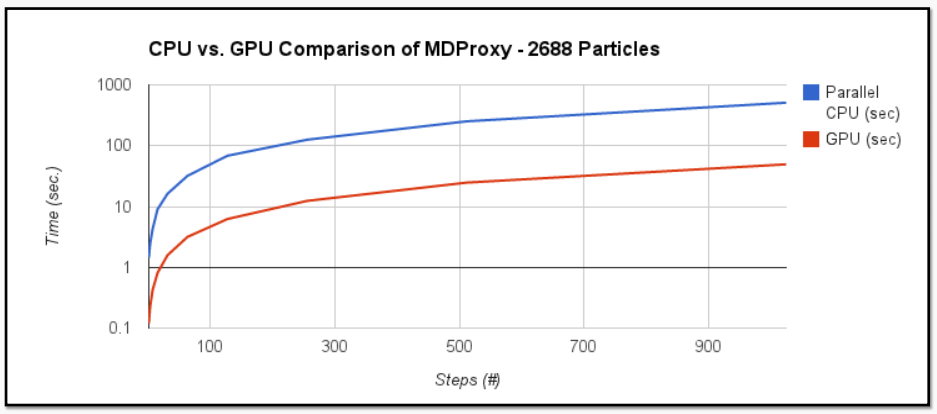
\includegraphics[width=8cm]{imgs/cpu_gpu.png}
\caption{MDProxy evaluation of the GPU vs. CPU implementations.}
\label{fig:cpu_gpu}
\end{figure}

\begin{figure}[h]
\centering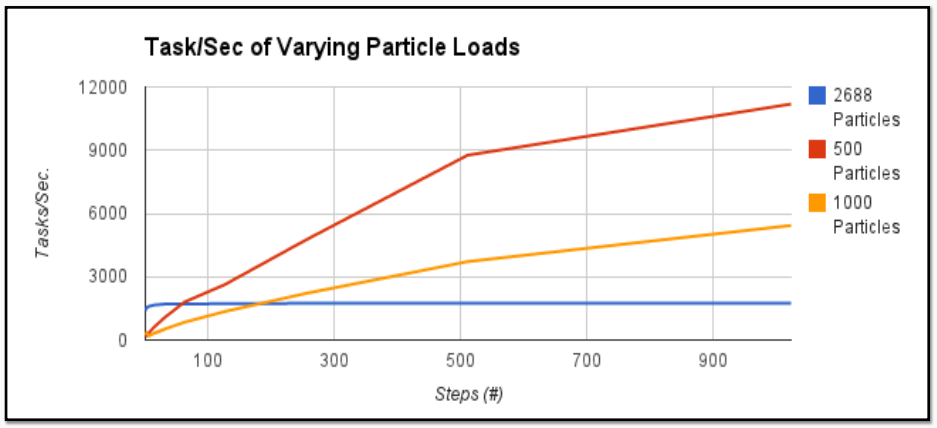
\includegraphics[width=8cm]{imgs/tasks_per_sec.png}
\caption{Tasks per second achieved during MDProxy.}
\label{fig:tasks_per_sec}
\end{figure}


\section{Conclusions}
In conclusion this work aimed to evaluate a real scientific application. While the MD code evaluated here is not a production code it provides a skeleton of data movement and compute that is performed by MD Codes. MDProxy highlights the GeMTC potential by launching small compute universes on each compute element in the GPU. Finally, our preliminary results show that GeMTC 10x faster than a threaded CPU implementation.

\section{Future Work}
Future work will aim to improve the MD algorithm, this will provide for a more through analysis of the potential improved performance that GeMTC can provide. We will also extend our evaluation by testing MDProxy at Multi-Node scale. MDProxy provides an array of input parameters that affect the computation, further investigation will aim to find optimal task sizes. Finally, we aim to compare performance against other GeMTC-enabled accelerators and develop high level abstractions for the Swift/T + GeMTC stack while Expanding the library of GeMTC microkernels.

\bibliographystyle{IEEEtran}
\bibliography{ref}
\end{document}
